\section{1174071 - Muhammad Abdul Gani Wijaya}

\subsection{Teori}
\begin{enumerate}
	\item Jelaskan kenapa file suara harus di lakukan MFCC. dilengkapi dengan ilustrasi atau gambar.
	\hfill\break
	Mel Frequency Cepstral Coefficient (MFCC) berguna untuk melakukan proses ekstraksi data khususnya audio dan juga merupakan suaut fitur yang ada di aplikasi pengenalan suara yang bisa digunakan untuk mengenali kata atau angka yang dikenal.
	\hfill\break
	\begin{figure}[H]
		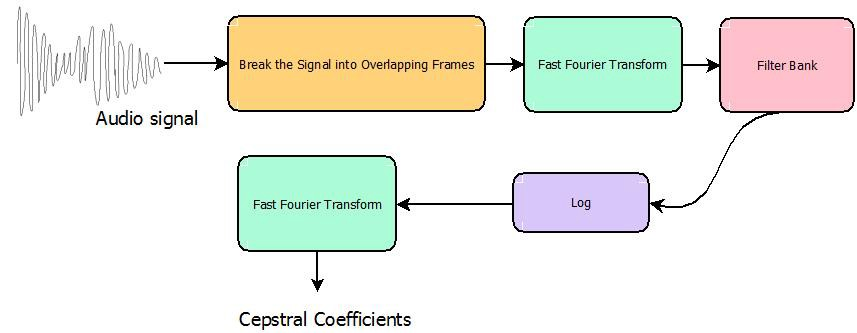
\includegraphics[width=8cm]{figures/1174071/6/mfcc.jpeg}
		\centering
	\end{figure}
	\item Jelaskan konsep dasar neural network.dilengkapi dengan ilustrasi atau gambar.
	\hfill\break
	Neural network merupakan suatu set algoritma yang dibuat berdasarkan otak manusia. didesain untuk mengenali pola, neural network mengintepresentasikan data sensor melalu berbagai macam persepsi mesin, melabeli atau mengelompokkan input. pola yang dapat dikenali dapat berupa angka atau vektor atau bisa juga data real seperti gambar atau suara dan juga teks.
	\hfill\break
	\begin{figure}[H]
		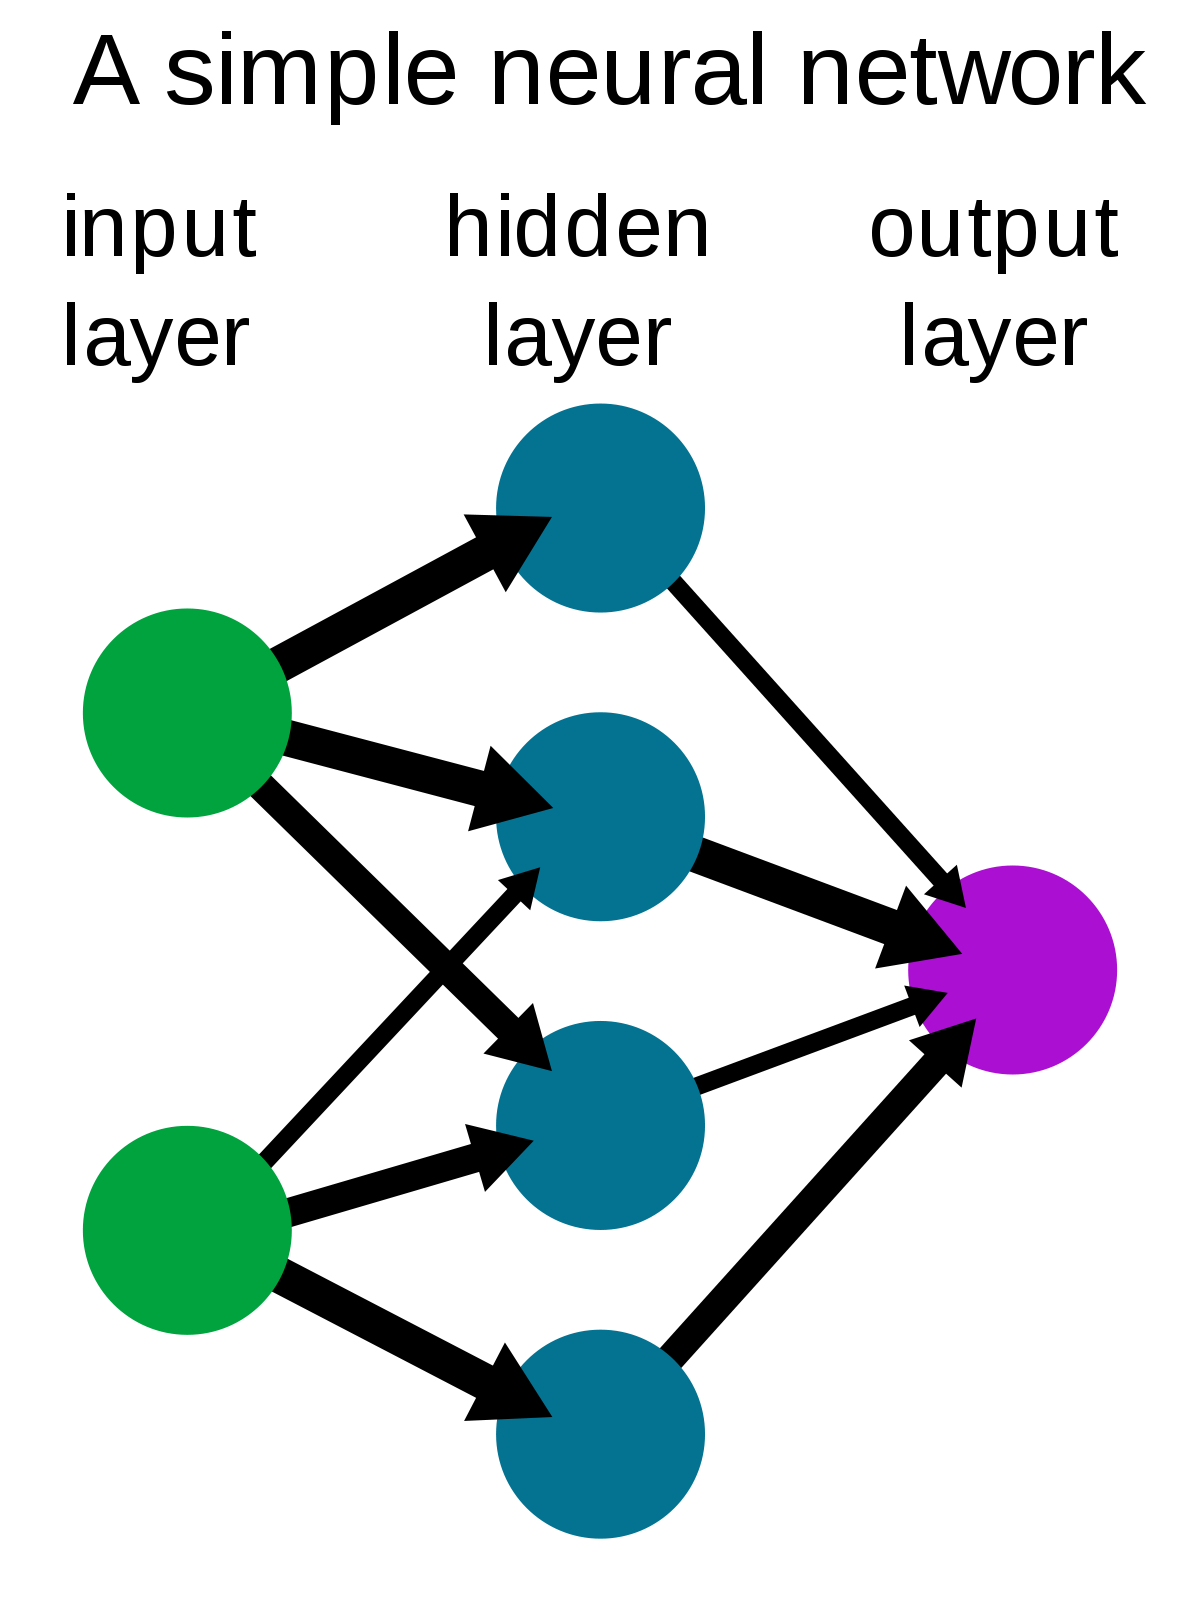
\includegraphics[width=8cm]{figures/1174071/6/neural.png}
		\centering
	\end{figure}
	\item Jelaskan konsep pembobotan dalam neural network. dilengkapi dengan ilustrasi atau gambar.
	\hfill\break
	Weight merupakan parameter dalam neural network yang berguna untuk melakukan transformasi data input yang akan masuk kebagian hidden layer dari neural network. suatu neural network merupakan sekelompok dari nodes atau neuron. di dalam tiap node ada beberapa set instruksi, bobot, dan juga bias value. suatu input masuk ke bagian node kemudian di jumlahkan dengan value dari weight dan hasilnya akan di lihat atau di berikan ke layer berikutnya yang ada pada neural network. seringkali bobot yang ada pada neural network sering berada pada bagian hidden layer di neural network
	\begin{figure}[H]
		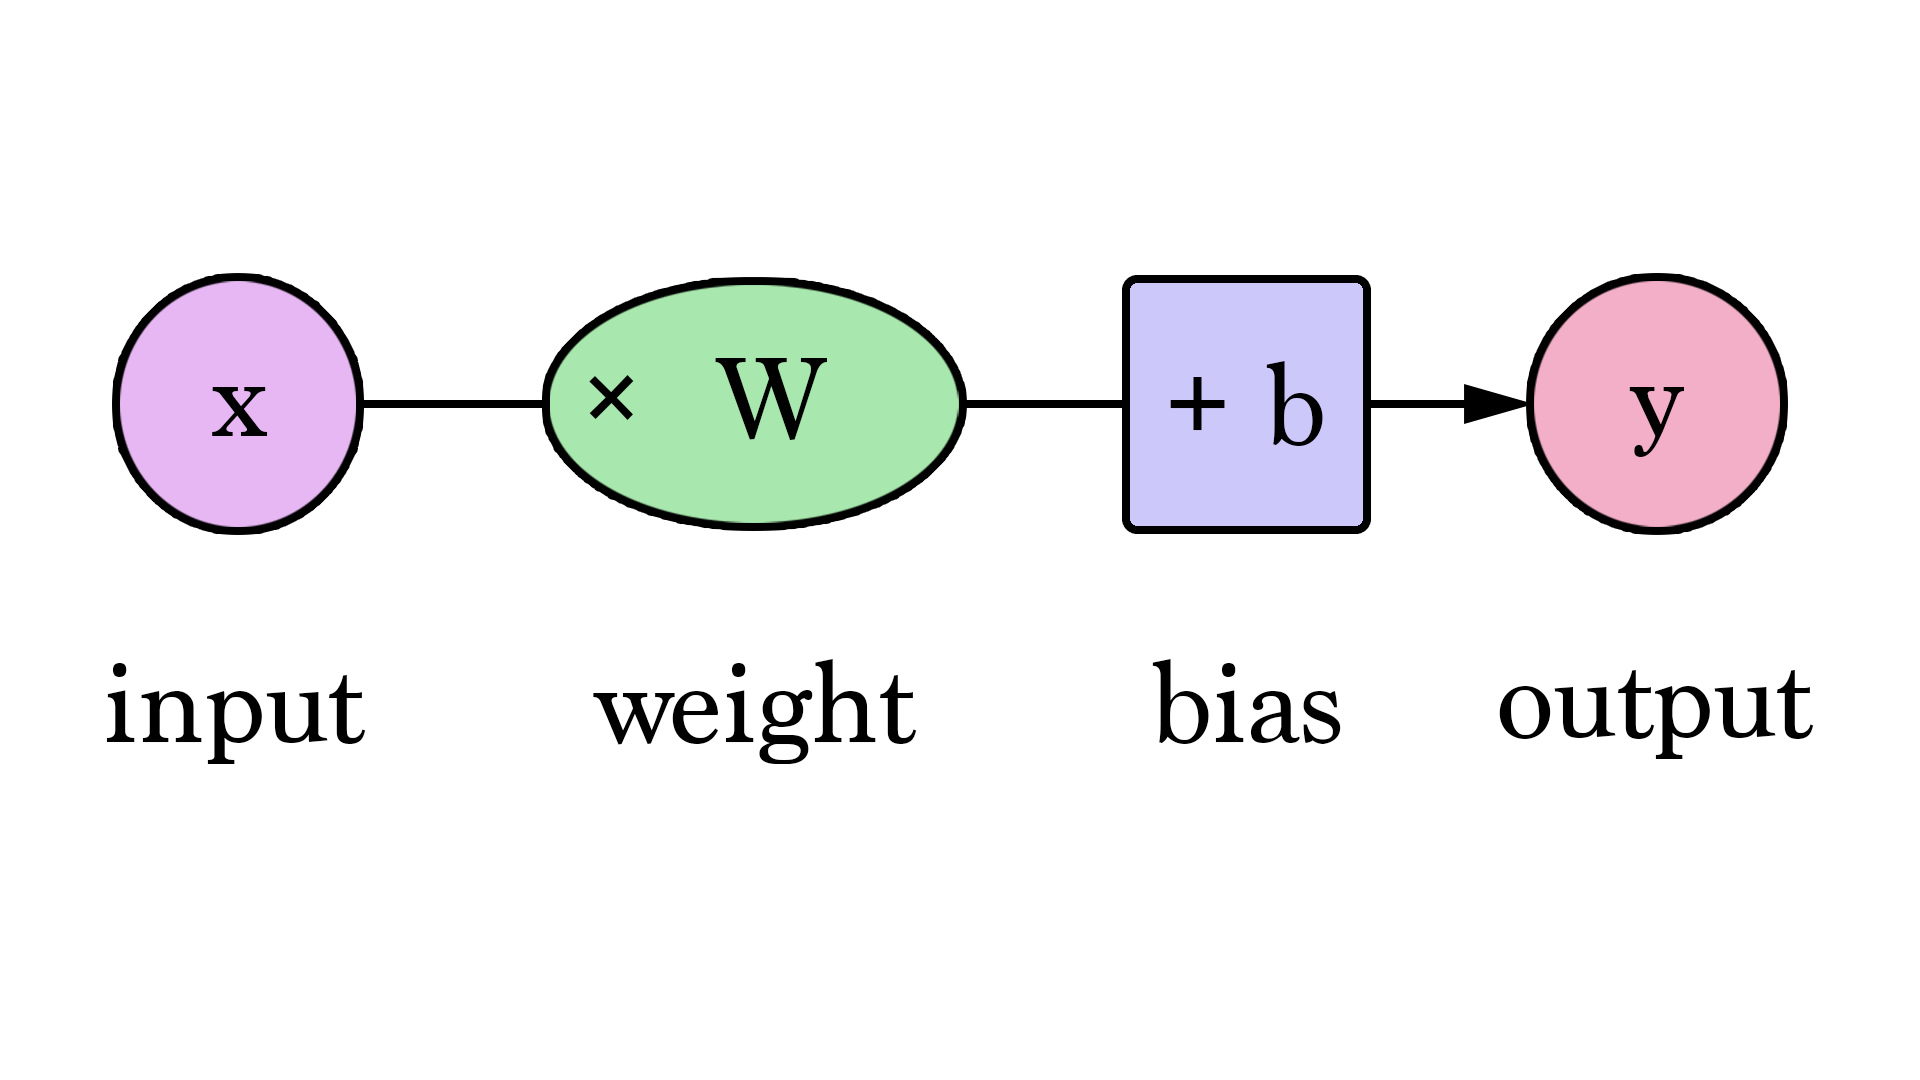
\includegraphics[width=8cm]{figures/1174071/6/weight.png}
		\centering
	\end{figure}
	\item Jelaskan konsep fungsi aktifasi dalam neural network.  dilengkapi dengan ilustrasi atau gambar.
	\hfill\break
	function aktifasi merupakan sebuah rumus matematika yang ada diantara input neuron dan output yang akan menuju ke layer berikutnya. Hal ini bisa sesimple seperti langkah langkah function yang  berfungsi untuk menyalakan atau mematikan suatu output dari neuron yang tergantung oleh beberapa aturan.
	\begin{figure}[H]
		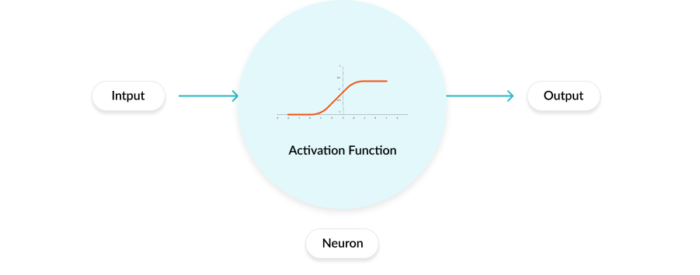
\includegraphics[width=8cm]{figures/1174071/6/aktifasi.png}
		\centering
	\end{figure}
	\item Jelaskan cara membaca hasil plot dari MFCC, dilengkapi dengan ilustrasi atau gambar.
	\hfill\break
	\begin{figure}[H]
		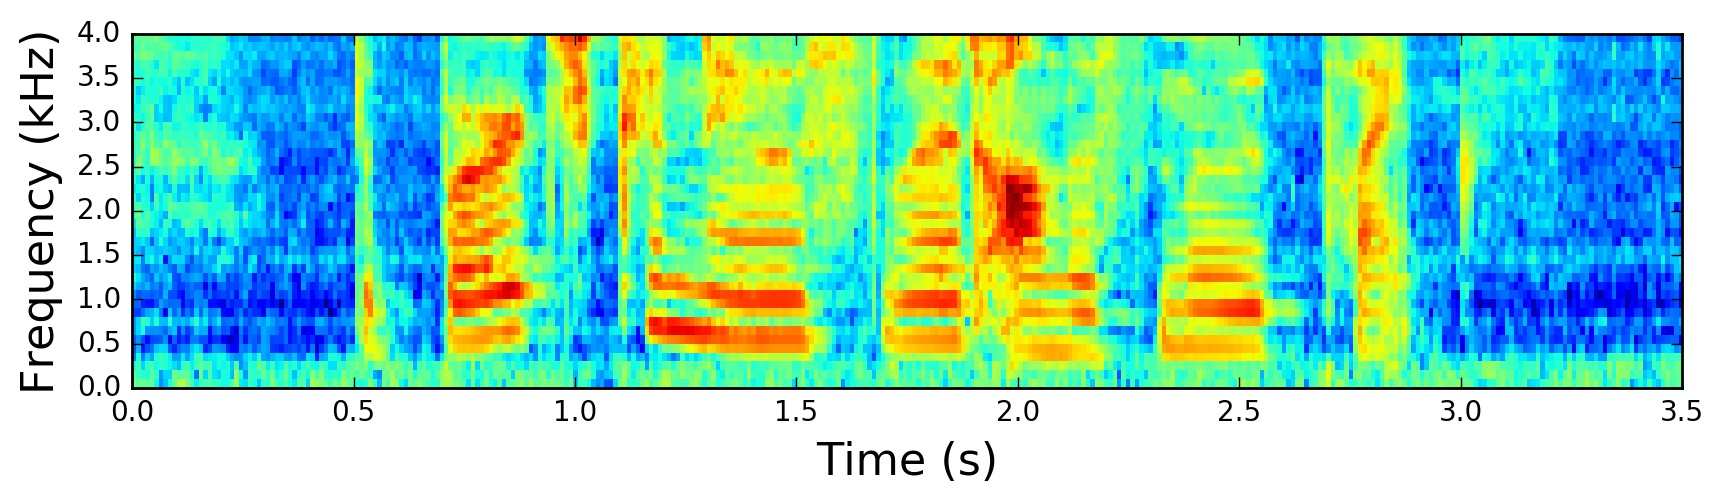
\includegraphics[width=8cm]{figures/1174071/6/mfccdiagram.jpg}
		\centering
	\end{figure}
	Sumbu y digunakan untuk mengukur tingginya khz, sementara sumbu x digunakan untuk mengukur durasi dari audio tersebut.
	\item Jelaskan apa itu one-hot encoding, dilengkapi dengan  ilustrasi kode dan atau gambar.
	One hot encoding digunakan untuk memisahkan columm yang berisi kategori berdasarkan angka menjadi ke beberapa columm berdasarkan jumlah kategori yang ada. setiap kolumm berisi 0 atau 1. one hot encoding dipakai untuk kasus kasus seperti misalkan pada suatu dataset, kita menemukan kolumm yang berisi angka tanpa suatu susunan. data ini biasanya menggambarkan kategori atau value dari suatu kategori. ini akan membuat machine learning kebingungan sehingga kita butuh yang namanya one hot encoding agar mesin mengerti.
	\begin{figure}[H]
		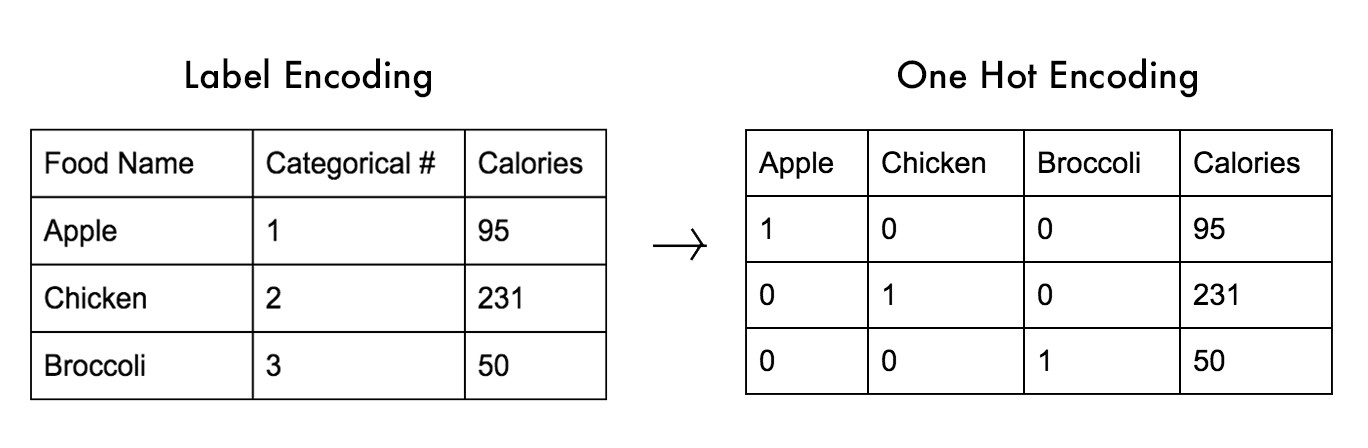
\includegraphics[width=8cm]{figures/1174071/6/onehot.jpg}
		\centering
	\end{figure}
	\item Jelaskan apa fungsi dari Sequential dalam kode program,dilengkapi dengan ilustrasi atau gambar.
	\hfill\break
	Sequential digunakan untuk membuat suatu prediksi dari data yang dinputkan. contohnya seperti gambar dibawah ini yang digunakan untuk memprediksi adjective, noun,verb dan pronoun dari teks bahasa inggris
	\begin{figure}[H]
		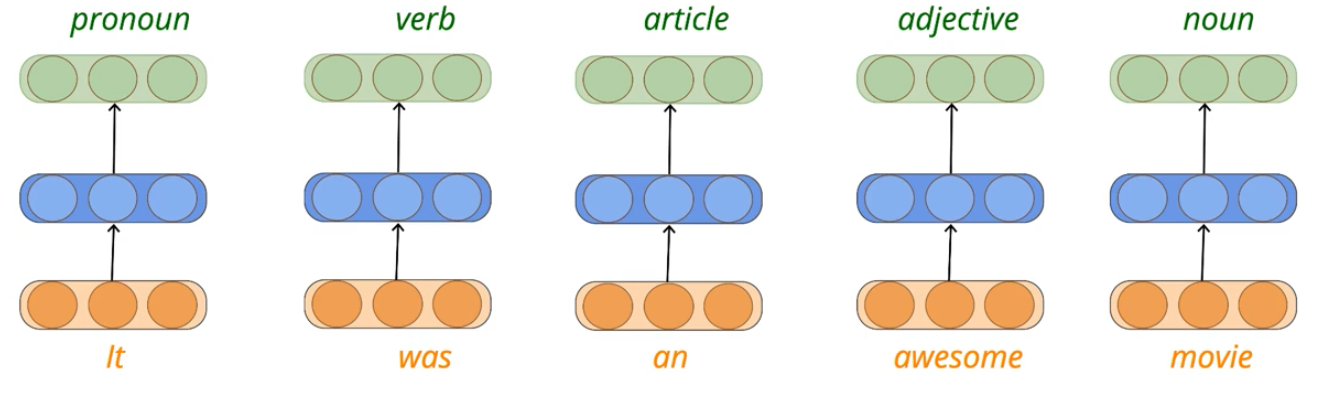
\includegraphics[width=8cm]{figures/1174071/6/sequential.png}
		\centering
	\end{figure}
\end{enumerate}

\subsection{Praktek}
\begin{enumerate}
	\item Jelaskan isi dari data GTZAN Genre Collection dan data dari freesound. Buat kode program untuk meload data tersebut untuk digunakan pada MFCC. Jelaskan arti dari setiap baris kode yang dibuat(harus beda dengan teman sekelas).
	\hfill\break
	\ GTZAN Genre Collection merupakan sebuah koleksi lagu dari berbagai jenis genre yang durasinya rata rata 30 detik.\\
	Data dari freesound yang chandra gunakan ada 2 yaitu kick.wav dan juga spaceysynth.wa.\\
	Kode program untuk meload data tersebut untuk digunakan pada MFCC.
	\lstinputlisting[firstline=8, lastline=36]{src/1174071/6/1174071.py}
	\hfill\break
	Import librarynya terlebih dahulu seperti librosa, glob dan numpy serta matplotlib dan juga keras. Librosa digunakan untuk ekstrak fitur yang ada pada lagu, glob digunakan untuk membuat list file, sedangkan numpy untuk melakukan operasi yang berhubungan dengan angka dan matplotlib untuk membuat grafik. import juga sequential dan lain lain dari library keras untuk penggunaan function activation serta dense yang memiliki banyak sekali neuron didalamnya serta tocategorical untuk merubah vector menjadi binary
	\hfill\break
	Setelah itu buat class dengan parameter bernama song yang isinya berisi function untuk load lagu dan fitur serta spectogramnya
	\hfill\break
	Berikut hasilnya
	\hfill\break
	\begin{figure}[H]
		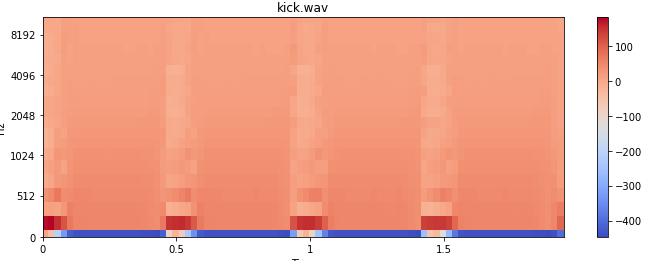
\includegraphics[width=8cm]{figures/1174071/6/1,1.PNG}
		\centering
	\end{figure}
	\hfill\break
	\begin{figure}[H]
		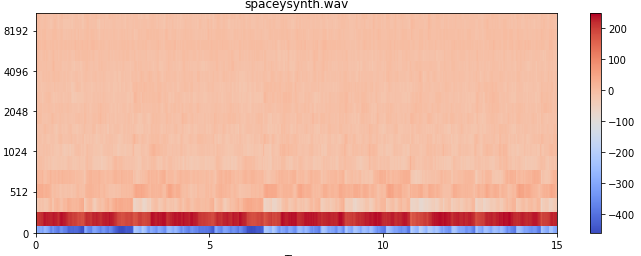
\includegraphics[width=8cm]{figures/1174071/6/1,2.PNG}
		\centering
	\end{figure}
	\hfill\break
	\begin{figure}[H]
		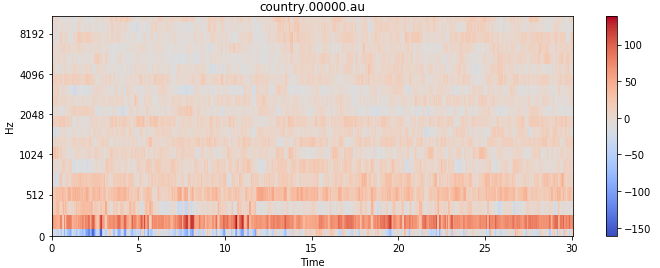
\includegraphics[width=8cm]{figures/1174071/6/1,3.PNG}
		\centering
	\end{figure}
	\hfill\break
	\begin{figure}[H]
		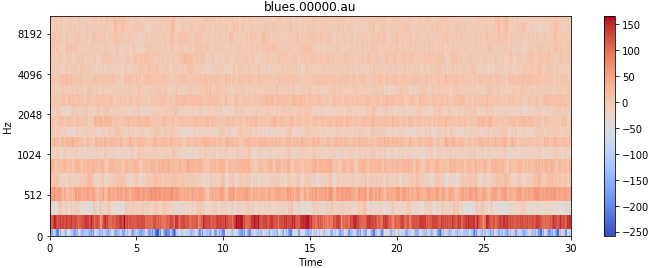
\includegraphics[width=8cm]{figures/1174071/6/1,4.PNG}
		\centering
	\end{figure}
	\item Jelaskan perbaris kode program dengan kata-kata dan dilengkapi ilustrasi gambar fungsi dari displaymfcc()
	\hfill\break
	\lstinputlisting[firstline=37, lastline=47]{src/1174071/6/1174071.py}
	\begin{itemize}
		\item Nama fungsinya adalah displaymfcc dengan satu parameter bernama song.
		\item Fungsi load() yang dipanggil digunakan untuk meload lagunya yang kemudian ditampung di variable.
		\item Fungsi mfcc() dipakai untuk melakukan ekstrak fitur file lagu yang dimuat kemudian ditampung pada variable nilainya.
		\item Fungsi figure() digunakan untuk membuat grafik.
		\item Fungsi specshow() untuk membuat spectogram
		\item Fungsi colorbar() digunakan untuk memberi warna pada grafik
		\item Fungsi title() untuk memberikan judul pada grafik.
		\item Fungsi tightlayout() untuk menyesuaikan layout grafik.
		\item Fungsi show() menampilkan output grafik.
	\end{itemize}
	Jika kita memanggil fungsi displaymfcc() nantinya akan seperti ini.
	\hfill\break
	\begin{figure}[H]
		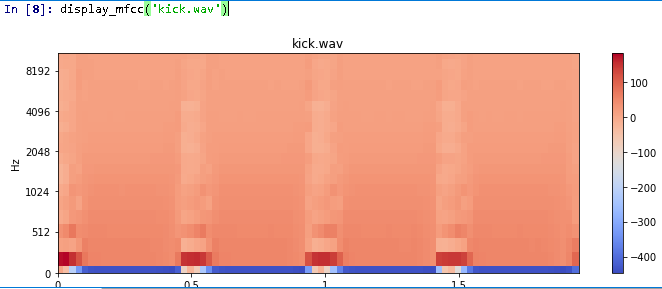
\includegraphics[width=8cm]{figures/1174071/6/2.PNG}
		\centering
	\end{figure}
	\item Jelaskan perbaris kode program dengan kata-kata dan dilengkapi ilustrasi gambar fungsi dari extractfeaturessong(). Jelaskan juga mengapa yang diambil 25.000 baris pertama?
	\hfill\break
	\lstinputlisting[firstline=49, lastline=57]{src/1174071/6/1174071.py}
	\begin{itemize}
		\item Pertama-tama nama fungsinya adalah extractfeaturessong dengan parameter bernama f
		\item Fungsi load() dipakai untuk memuat lagunya yang kemudian disimpan di variable.
		\item Fungsi mfcc() untuk melakukan ekstrak fitur file lagu yang dimuat lalu disimpan nilainya di variable.
		\item Fungsi absolute() digunakan supaya nilainya menjadi nilai absolut. Sedangkan fungsi amax dipakai untuk mencari nilai max. Lalu hasil yang didapatkan sebelumnya dibagi dengan nilai mfcc.
		\item Terakhir, hasil yang telah ditampung di variable mfcc di convert ke array 1 dimensi dan diambil 25000 baris pertama saja mengembalikan hasil convert array ke dalam bentuk satu dimensi dari nilai mfcc dan diambil 25000 baris pertama.
		\item Alasannya mengapa hanya diambil 25000 baris pertama karena hampir setiap lagu memiliki durasi atau panjang yang berbeda beda sementara data yang harus dimasukan ke machine learning harus ukuran yang sama.
	\end{itemize}
	\hfill\break
	\begin{figure}[H]
		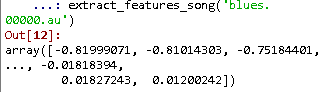
\includegraphics[width=8cm]{figures/1174071/6/3.PNG}
		\centering
	\end{figure}
	\item Jelaskan perbaris kode program dengan kata-kata dan dilengkapi ilustrasi gambar fungsi dari generatefeaturesandlabels().
	\hfill\break
	\lstinputlisting[firstline=60, lastline=78]{src/1174071/6/1174071.py}
	\begin{itemize}
		\item Buat fungsi dengan nama generatefeaturesandlabels().
		\item Kemudian buat array list allfeatures
		\item Kemudian buat array list alllabels
		\item Lalu buat array list genres untuk menyimpan daftar genre musik
		\item Gunakan loop untuk melakukan proses secara berulang agar semua file dapat dimuat
		\item Pakai fungsi glob() untuk mencari file lagu yang ingin dimuat dengan mendefinisikan direktorinya
		\item Memperlihatkan panjang daftar lagu berdasarkan genre
		\item looping pada soundfiles
		\item Gunakan fungsi extractfeaturessong() untuk mengambil fitur yang ada pada file musik yang di load
		\item tambahkan hasil dari fungsi extractfeaturessong() ke allfeatures
		\item Isi allfeatures dengan features dan alllabels dengan genrelabels
		\item Gunakan fungsi unique untuk membuat label unik
		\item Gunakan fungsi astype untuk mengubah type menjadi type int32
		\item Gunakan function tocategorical untuk melakukan konversi ke one-hot-encoding
		\item Return nilainya kemudian gabungkan dengan fungsi stack() dari allfeatures ke matrix
		\item panggil fungsinya
	\end{itemize}
	\hfill\break
	\begin{figure}[H]
		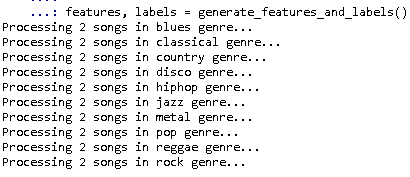
\includegraphics[width=8cm]{figures/1174071/6/4.png}
		\centering
	\end{figure}
	\item Jelaskan dengan kata dan praktek kenapa penggunaan fungsi generatefeaturesandlabels() sangat lama ketika meload dataset  genre. Tunjukkan keluarannya dari komputer sendiri dan artikan maksud setiap luaran yang didapatkan.
	\hfill\break
	Sangat lama karena file yang dimuat bisa banyak yaitu ada 1000 file serta kita juga mencari 25000 nilai pertama dari setiap file yang ada sehingga akibatnya lama, apabila hanya dua file seperti gambar dibawah ini tentunya lebih cepat.
	\hfill\break
	\begin{figure}[H]
		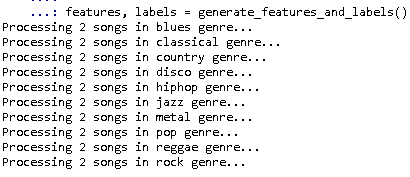
\includegraphics[width=8cm]{figures/1174071/6/4.png}
		\centering
	\end{figure}
	\item Jelaskan kenapa harus dilakukan pemisahan data training dan data set sebesar 80 persen? Praktekkan dengan kode dan Tunjukkan keluarannya dari komputer sendiri dan artikan maksud setiap luaran yang didapatkan.
	\hfill\break
	Karena agar nantinya data yang akan kita hitung menghasilkan hasil yang lebih akurat dan juga meminimalisir kemungkinan kesalahan oleh mesinnnya itu sendiri.
	\lstinputlisting[firstline=80, lastline=95]{src/1174071/6/1174071.py}
	\hfill\break
	\begin{figure}[H]
		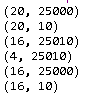
\includegraphics[width=8cm]{figures/1174071/6/6.PNG}
		\centering
	\end{figure}
	\begin{itemize}
		\item Ukuran array atau jumlah data pada data features
		\item Ukuran array atau jumlah data pada data labels
		\item Ukuran array atau jumlah data pada data train
		\item Ukuran array atau jumlah data data test
		\item Ukuran array atau jumlah data data traininput
		\item Ukuran array atau jumlah data data trainlabels
	\end{itemize}
	\item Praktekkan dan jelaskan masing-masing parameter dari fungsi Sequential(). Tunjukkan keluarannya dari komputer sendiri dan artikan maksud setiap luaran yang didapatkan.
	\hfill\break
	\lstinputlisting[firstline=97, lastline=102]{src/1174071/6/1174071.py}
	Layer pertama terdapat 100 neuron dengan parameter berjumlah 25000 yang didapat dari variable train input dengan neuron sebanyak 100, layer kedua memiliki 10 neuron dengan parameter sekitar 1010 input ditambah biasnya 10. Dengan total params 2501110. Setelah itu data dilakukan training.
	\begin{itemize}
		\item Layer pertama adalah layer dense dengan jumlah 100 neuron, kemudian inputkan datanya
		\item Eksekusi activation dengan tipe relu
		\item Lalu ada layer kedua dengan jumlah sebanyak 10 neuron
		\item Melakukan fungsi activation dengan tipe softmax
	\end{itemize}
	\hfill\break
	\begin{figure}[H]
		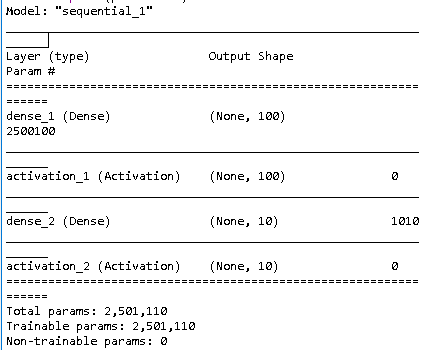
\includegraphics[width=8cm]{figures/1174071/6/7.PNG}
		\centering
	\end{figure}	
	\item Praktekkan dan jelaskan masing-masing parameter dari fungsi compile(). Tunjukkan keluarannya dengan fungsi summary dari komputer sendiri dan artikan maksud setiap luaran yang didapatkan.
	\hfill\break
	\lstinputlisting[firstline=103, lastline=105]{src/1174071/6/1174071.py}

	\begin{itemize}
		\item Optimizer yang dipakai yaitu adam
		\item Loss dipakai adalah categoricalcrosssentropy
		\item Metrics yang dipakai accuracy
	\end{itemize}
	\hfill\break
	\begin{figure}[H]
		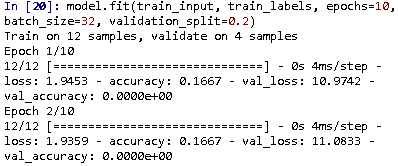
\includegraphics[width=8cm]{figures/1174071/6/7,1.PNG}
		\centering
	\end{figure}
	Layer pertama terdapat 100 neuron dengan parameter berjumlah 25000 yang didapat dari variable train input dengan neuron sebanyak 100, layer kedua memiliki 10 neuron dengan parameter sekitar 1010 input ditambah biasnya 10. Dengan total params 2501110.
	\item  Praktekkan dan jelaskan masing-masing parameter dari fungsi fit().Tunjukkan keluarannya dari komputer sendiri dan artikan maksud setiap luaran yang didapatkan.
	\hfill\break
	\lstinputlisting[firstline=107, lastline=108]{src/1174071/6/1174071.py}
	\begin{itemize}
		\item Parameter yang pertama adalah variable train input
		\item Parameter yang pertama adalah variable train labels
		\item Jumlah epoch yang dipakai adalah 10
		\item Batch Size yang dipakai sebesar 32
		\item Validation Splitnya adalah 0.2 atau 20\%
	\end{itemize}
	\hfill\break
	\begin{figure}[H]
		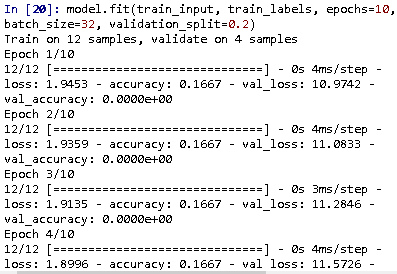
\includegraphics[width=8cm]{figures/1174071/6/9.PNG}
		\centering
	\end{figure}
	\item Praktekkan dan jelaskan masing-masing parameter dari fungsi evaluate(). Tunjukkan keluarannya dari komputer sendiri dan artikan maksud setiap luaran yang didapatkan.
	\hfill\break
	\lstinputlisting[firstline=110, lastline=112]{src/1174071/6/1174071.py}
	\begin{itemize}
		\item Parameter yang pertama adalah variable test input
		\item Parameter yang kedua adalah variable test labels
		\item Batch Size yang dibutuhkan 32
	\end{itemize}
	\hfill\break
	\begin{figure}[H]
		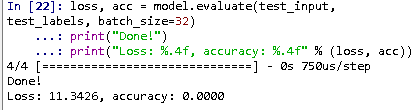
\includegraphics[width=8cm]{figures/1174071/6/10.PNG}
		\centering
	\end{figure}
	Lossnya 11.3426,dan akurasinya 0.000
	\item Praktekkan dan jelaskan masing-masing parameter dari fungsi predict(). Tunjukkan keluarannya dari komputer sendiri dan artikan maksud setiap luaran yang didapatkan.
	\hfill\break
	\lstinputlisting[firstline=114, lastline=115]{src/1174071/6/1174071.py}
	\begin{itemize}
		\item Parameter yang pertama adalah variable test input
		\item Batch Size yang dibutuhkan 32
	\end{itemize}
	\hfill\break
	\begin{figure}[H]
		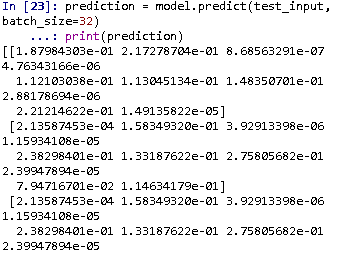
\includegraphics[width=8cm]{figures/1174071/6/11.PNG}
		\centering
	\end{figure}
\end{enumerate}

\subsection{Penanganan Error}
No module named librosa
\subsubsection{Solusi Error}
\begin{figure}[H]
		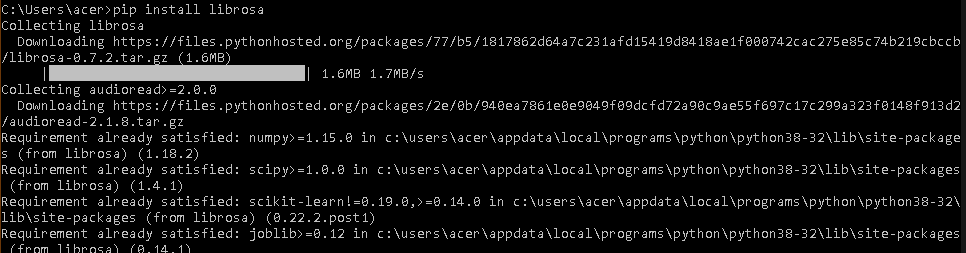
\includegraphics[width=8cm]{figures/1174071/6/error.PNG}
		\centering
	\end{figure}
Install library terlebih dahulu
\subsection{Bukti Tidak Plagiat}
\begin{figure}[H]
	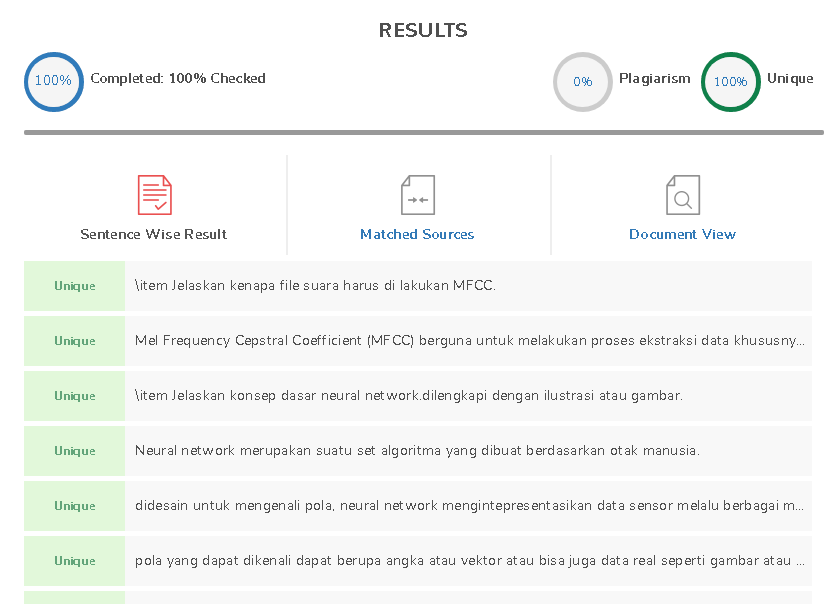
\includegraphics[width=8cm]{figures/1174071/6/plagiat.PNG}
	\centering
\end{figure}
\subsection{Link Youtube}
https://youtu.be/VE-lHR3L9zw